\documentclass[10pt, final, hyperref, table]{beamer}
\mode<presentation>


 %\usepackage[english]{babel} % "babel.sty"
% \usepackage{french}                  % "french.sty"
%  \usepackage{franglais}               % "franglais.sty" (a defaut)
  \usepackage{times}            % ajout times le 30 mai 2003
 
%% --------------------------------------------------------------
%% CODAGE DE POLICES ?
%% Si votre moteur Latex est francise, il est conseille
%% d'utiliser le codage de police T1 pour faciliter la césure,
%% si vous disposez de ces polices (DC/EC)
\usepackage[utf8]{inputenc}
\usepackage[T1]{fontenc}
\usepackage{eurosym}


%% ==============================================================
%\usepackage{graphicx}
\usepackage{amsmath,amsfonts}
%\usepackage[table]{xcolor}
\usepackage{subfigure}
\usepackage{fancybox}

\usepackage{multicol}
\usepackage{wrapfig}
\usepackage{listings}
\usepackage{xcolor}
\usepackage{multimedia} % For playing sound

\usepackage{hyperref}
% Define hyperlinks color
\definecolor{links}{HTML}{2A1B81}
\hypersetup{colorlinks,linkcolor=,urlcolor=links}

\usetheme{Madrid}
\setbeamercovered{transparent}


% telemeta red
\definecolor{telemetaRed}{rgb}{0.41568, 0.01176, 0.02745}   % #6A0307
\usecolortheme[rgb={0.41568, 0.01176, 0.02745}]{structure} 

%\setbeamercolor{frametitle}{bg=telemetaRed}
% Display a grid to help align images
%\beamertemplategridbackground[1cm]

%We will get the normal bibliography style (number or text instead of icon) by including the following code
\setbeamertemplate{bibliography item}[text]
\setbeamerfont{caption}{size=\footnotesize}
% listings settings
\definecolor{lstComments}{rgb}{0,0.6,0}
\definecolor{lstBkgrd}{rgb}{0.95,0.95,1}
\lstset{%
  language=Python, % the language of the code
  frame=single,  % adds a frame around the code
  frameround=tttt,
  commentstyle=\color{lstComments},% comment style
  backgroundcolor=\color{lstBkgrd},   % choose the background color
  basicstyle=\tiny,       % the size of the fonts that are used for the code
  stringstyle=\ttfamily,  % typewriter type for strings
  keywordstyle=\color{blue},      % keyword style
  showstringspaces=false,          % underline spaces within strings only
}


\definecolor{rouge}{rgb}{1.0,0,0}
\newcommand{\chref}[2]{
    \href{#1}{\color{rouge}\underline{#2}}
}
\newcommand{\dchref}[1]{
    \href{#1}{\color{rouge}\underline{#1}}
}
\newcommand{\curl}[1]{
    \color{rouge}\underline{\url{#1}}
}
\title[TimeSide, open web audio processing framework]{
    TimeSide\\
    An open web audio processing framework
    }

%\author{Guillaume Pellerin\inst{1}}

\author[G. Pellerin, T. Fillon, P. Brossier]{
  Guillaume Pellerin\inst{1},
  Thomas Fillon\inst{1,2},
  Paul Brossier\inst{1},
}


\institute[Parisson/UPMC]{%
  \inst{1}%
  Parisson, Paris, France 
  \and%
  \inst{2}%
  LAM, Institut Jean Le Rond d'Alembert, UPMC Univ. Paris 06,  UMR CNRS 7190
 \begin{center}
   \includegraphics[height=0.6cm]{img/parisson_logo_FINALE_com.pdf}
   \hfill
   \includegraphics[width=0.3\textwidth]{img/logo_telemeta_1-1.pdf}
   \hfill
   \includegraphics[height=0.6cm]{img/upmc.png}
 \end{center}
}

\date[SoundSoftware Workshop - 8/07/2014]{SoundSoftware Workshop - 8/07/2014\\

\includegraphics[width=0.5\paperwidth]{img/soundsoftware_ac_uk_subtitle_transparent.png}}


\begin{document}
\frame{\titlepage}
\section[Table of contents]{}
\frame{\frametitle{Table of contents}
\tableofcontents
}

\section{The Telemeta Project}  
\subsection{Goals}

\begin{frame}\footnotesize
\frametitle{The Telemeta Project}

    \begin{columns}
      \begin{column}{0.5\linewidth}
        \includegraphics[width=4cm]{img/logo_telemeta_1-1.pdf}
      \end{column}
      \begin{column}{0.5\linewidth}
        \colorbox{yellow!50}{\textbf{\url{http://telemeta.org/}}}
      \end{column}
    \end{columns}
    \begin{block}{Main goals}
      \begin{itemize}
      \item \alert{Archive}, \alert{preserve} and \alert{manage} large
        audio database and related metadata
      \item \alert{Play} audio data and \alert{read} metadata
        \alert{synchronously}
      \item \alert{Process} audio data \alert{on demand} through a
        \alert{modular architecture} (no pre-processing needed)
      \item \alert{Index} and \alert{share} audio data through a
        \alert{collaborative} web app
      \item \alert{Link} audio data to various \alert{ontologies},
        external \alert{services} and related \alert{multimedia files}
      \item \alert{Manage} users, share and access rules, copyrights
        easily through time
      \end{itemize}
    \end{block}
    \begin{block}<2>{History of the project}
      \begin{itemize}
      \item \alert{2006}: Define objectives = \emph{open source web
          audio collaborative platform}
      \item \alert{2007}: First partner: french Center for Research in
        Ethnomusicology (CREM)
      \item \alert{2011}: Release of \alert{Telemeta 1.0} and
        deployment of the ``\emph{Sound archives of the CNRS
          - Musée de l'Homme}'' \dchref{http://archives.crem-cnrs.fr}
      \item \alert{2013 - 2014}: Provide audio processing capabilities through the DIADEMS project 
      \end{itemize}
    \end{block}
  
\end{frame}


\subsection{CREM's platform}
\begin{frame}
  \frametitle{CREM's platform}
  \begin{center}
    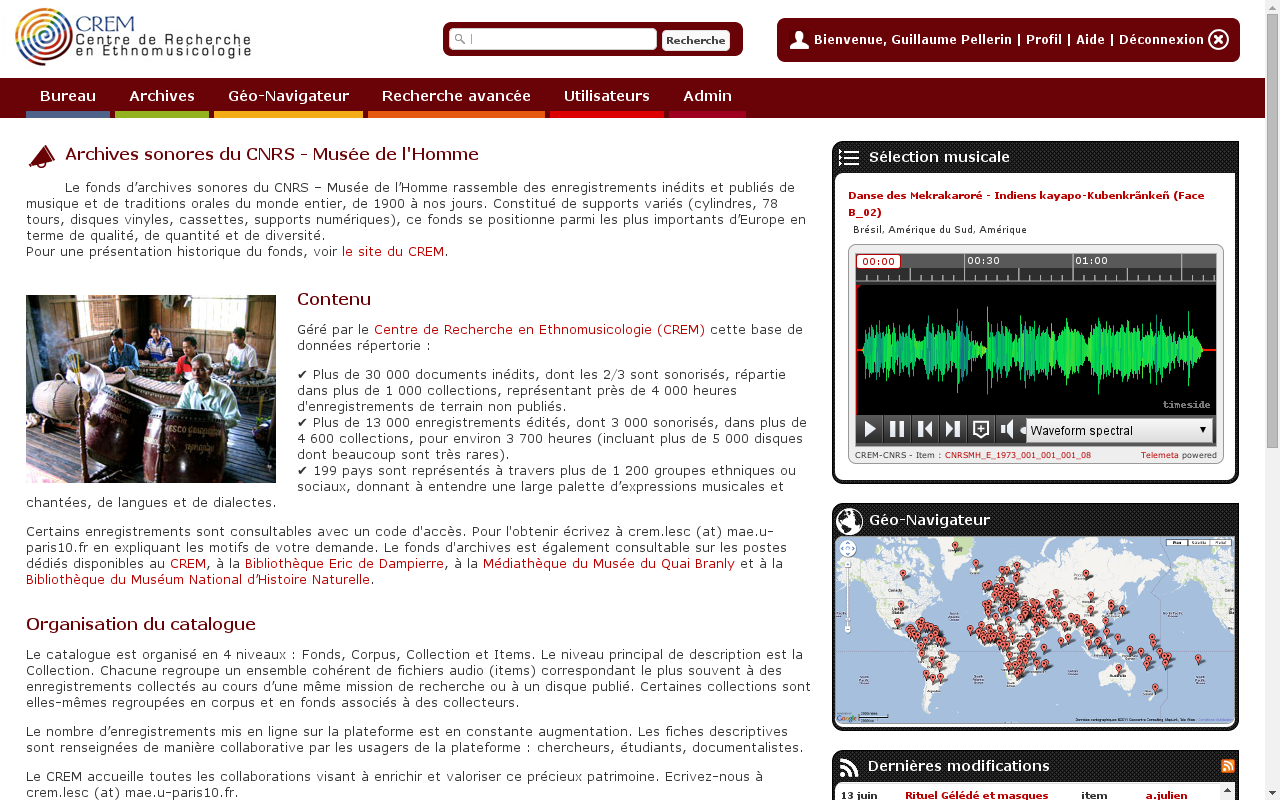
\includegraphics[width=\textwidth]{img/shots/CREM_2014_1.png}
  \end{center}
\end{frame}

\begin{frame}\frametitle{Telemeta - Web UI}
  \vspace{-0.25cm}
  \begin{center}
    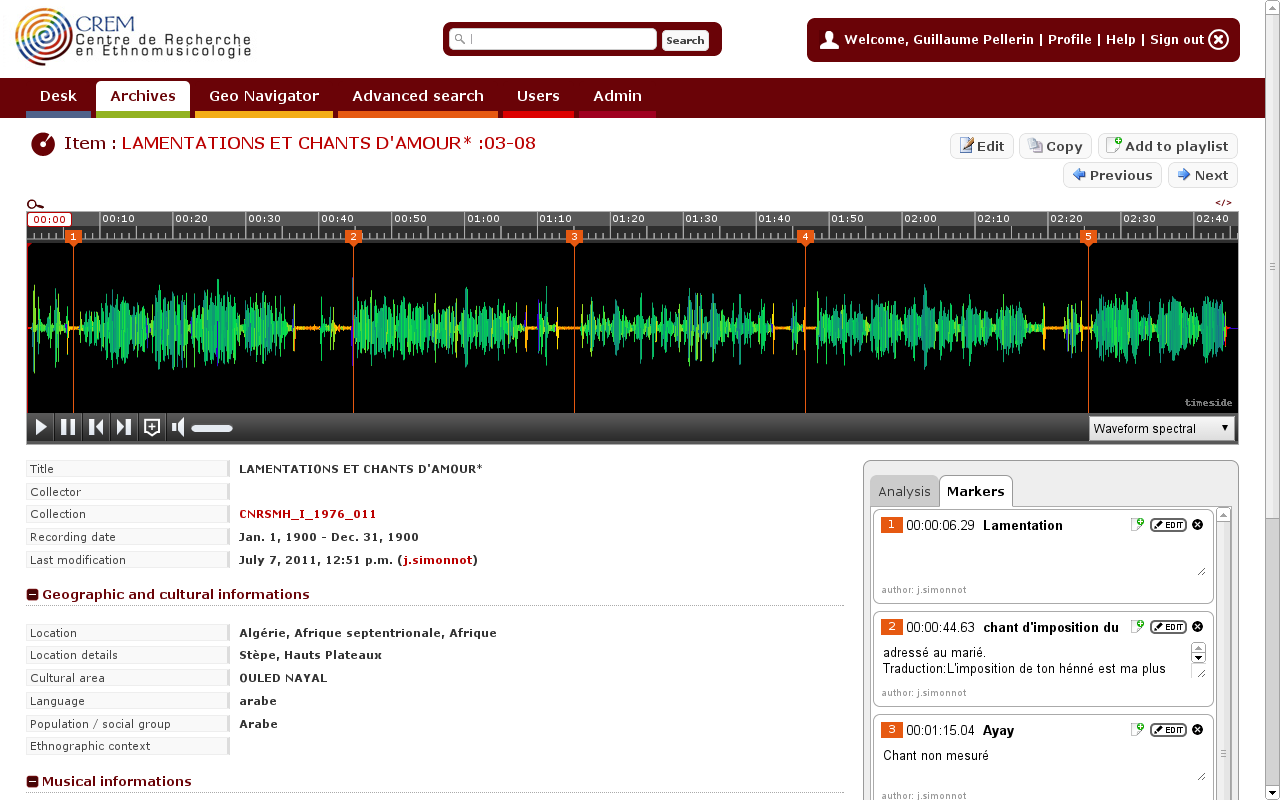
\includegraphics[width=12cm]{img/shots/telemeta_eng.png}
  \end{center}
  \tiny{\url{http://archives.crem-cnrs.fr/archives/items/CNRSMH_I_1976_011_003_08/}}
\end{frame}



\subsection{Technologies \& Key features}
\frame{\frametitle{Telemeta - Technologies \& Key features}
\footnotesize
\begin{block}{Technologies  \alert{$\longrightarrow$ 100\% 0pen Source!}}
 \begin{itemize}
 \item GNU / Linux : applications, libraries and kernel 
 \item \chref{http://python.org}{Python} (cool and smart object oriented language with web and scientific libraries), \chref{http://djangoproject.com}{Django} (web platform, \chref{http://gstreamer.freedesktop.org/}{GStreamer} (multimedia framework)
 \item MySQL, PostgreSQL, others : relational databases
 \item \chref{https://github.com/yomguy/TimeSide}{TimeSide} : open web audio processing framework 
\end{itemize}
\end{block}
\begin{block}{Key features}
  \begin{itemize}
  \item \alert{Pure HTML5} web user interface including dynamical
    forms and smart workflows
  \item \alert{On the fly} audio analyzing, transcoding and metadata
    embedding in various formats
  \item \alert{Social editing} with \alert{semantic ontologies}, smart
    workflows, realtime tools, human or automatic \alert{annotations
      and segmentations}
  \item \alert{User management} with individual desk, playlists,
    profiles and access rights
  \item \alert{High level search engine} (geolocation, instruments,
    ethnic groups, etc...)
  \item \alert{Data providers} : DublinCore, OAI-PMH, RSS, XML, JSON
    and other
  \item \alert{Multi-language} support (now english and french)
  \end{itemize}
\end{block}
}


\subsection{Architecture}
\frame{\frametitle{Telemeta - Architecture}
    \begin{center}
    \pgfimage[width=8cm]{img/TM_arch}
    \end{center}
}


\section{Goals}

\begin{frame}
 \frametitle{TimeSide - Goals}%\scriptsize
\begin{block}{Server side - TimeSide Engine}
  \begin{itemize}
  \item \alert{Do} asynchronous and fast audio processing with Python,
  \item \alert{Decode} audio frames from ANY format into numpy arrays,
  \item \alert{Analyze} audio content with state-of-the-art audio feature extraction libraries (Aubio, Yaafe, Vamp (experimental),
  \item  \alert{Organize}, serialize and save analysis metadata through various formats,
  \item  \alert{Draw} various fancy waveforms, spectrograms and other cool graphers,
  \item  \alert{Transcode} audio data in various media formats and stream them through web apps,
  \end{itemize}
 
\end{block}
\begin{block}{Client side - TimeSide UI}
  \begin{itemize}
  \item   \alert{Playback} and  \alert{interact} on demand through a smart high-level HTML5 extensible player,
  \item   \alert{Index},  \alert{tag} and  \alert{organize semantic metadata} \\
(see \href{http://telemeta.org/}{Telemeta} which embeds TimeSide). 
\hfill $\vcenter{\hbox{\includegraphics[width=0.2\textwidth]{img/logo_telemeta_1-1.pdf}}}$
 % \begin{flushright}
 %   
\includegraphics[width=0.2\textwidth]{../../Common/img/logo_telemeta_1-1.pdf}\\
 %   \colorbox{yellow!50}{\textbf{\url{http://telemeta.org/}}}
  %\end{flushright}
  \end{itemize}
\end{block}
\end{frame}


\section{Use cases}

\subsection{General}

\frame{\frametitle{Use cases}

    \begin{block}{Usages}
        \begin{itemize}
        \item Analyze large music audio datasets on demand over a robust and scalable platform
        \item Share audio data and metadata with experts to make them collaborate in editing, processing and discovering
        \item Build large statistical campaigns and vizualizations from ontologies, geographic data and sounds
        \item Scale the audio data through the web (URL indexes)
       \end{itemize}
    \end{block}
    
    \begin{block}<2>{Applications}
         \begin{itemize}
            \item Realtime bioacoustical monitoring system over internet (needs hardware)
            \item Biodiversity studies
            \item Development and test of new species detection algorithms on large and historical datasets
         \end{itemize}
    \end{block}
}



\subsection{The DIADEMS project}
\frame{\frametitle{The DIADEMS project}
\begin{itemize}
    \item \chref{http://www.irit.fr/recherches/SAMOVA/DIADEMS/fr/welcome/&cultureKey=en}{DIADEMS} : Description, Indexation, Access to Sound and Ethnomusicological Documents
    \item Granted by ANR : french national research agency (ANR-12-CORD-0022)     
    \item 3 years, 8 partners, 850 k\euro
    \item Apply and test MIR algorithms on large scale ethnomusicological data
    \item Define some high level interfaces to find new ways of explorations in large complex musical corpus
    \item New modes of collaboration between human science and computer science laboratories and researchers
    \item Define the \chref{http://files.parisson.com/telemeta/telemeta-doc/DIADEMS/thesaurus/Thesaurus/Thesaurus.html}{vocabulary} describing musical events in the usecase of ethnomusicilogy vs. signal processing
    \item \dchref{http://www.irit.fr/recherches/SAMOVA/DIADEMS/fr/welcome/}
    \item \dchref{http://diadems.telemeta.org}
\end{itemize}
}

\frame{\frametitle{DIADEMS - Partners}
\begin{itemize}
\item Sponsors:
\begin{itemize}
 \item CNRS
 \item Huma-Num (ex TGE Adonis)
 \item ANR
 \item CREM
 \item UPMC
 \item Parisson
\end{itemize}

\vspace{0.25cm}

\item Partners :
\begin{itemize}
\item IRIT (université Paul Sabatier, Toulouse 3)
\item LIMSI (universités Pierre et Marie Curie (UPMC, Paris 6) et Paris-Sud)
\item LAM (institut Jean Le Rond d'Alembert, UPMC)
\item LABRI (université de Bordeaux)
\item CREM (université Paris Ouest Nanterre La Défense)
\item LESC (université Paris Ouest Nanterre La Défense)
\item Museum d'Histoire Naturelle de Paris
\item Musée du Quai Branly
\end{itemize}

\end{itemize}

\begin{center}
\begin{columns}[c]
\column{2.5cm}
\begin{center}
\pgfimage[width=1cm]{img/logo-CNRS}\end{center}
\column{2.5cm}
\begin{center}
\pgfimage[width=2.5cm]{img/Logo-CREM-La.jpg}
\end{center}
\column{2.5cm}
\begin{center}
\pgfimage[width=2.5cm]{img/parisson_logo_200}\end{center}
\column{2cm}
\begin{center}
\pgfimage[width=1.2cm]{img/logo-mnhn}\end{center}
\end{columns}
\end{center}

}



\section{Architecture}

\begin{frame}
  \frametitle{TimeSide - Architecture}
  \begin{center}
    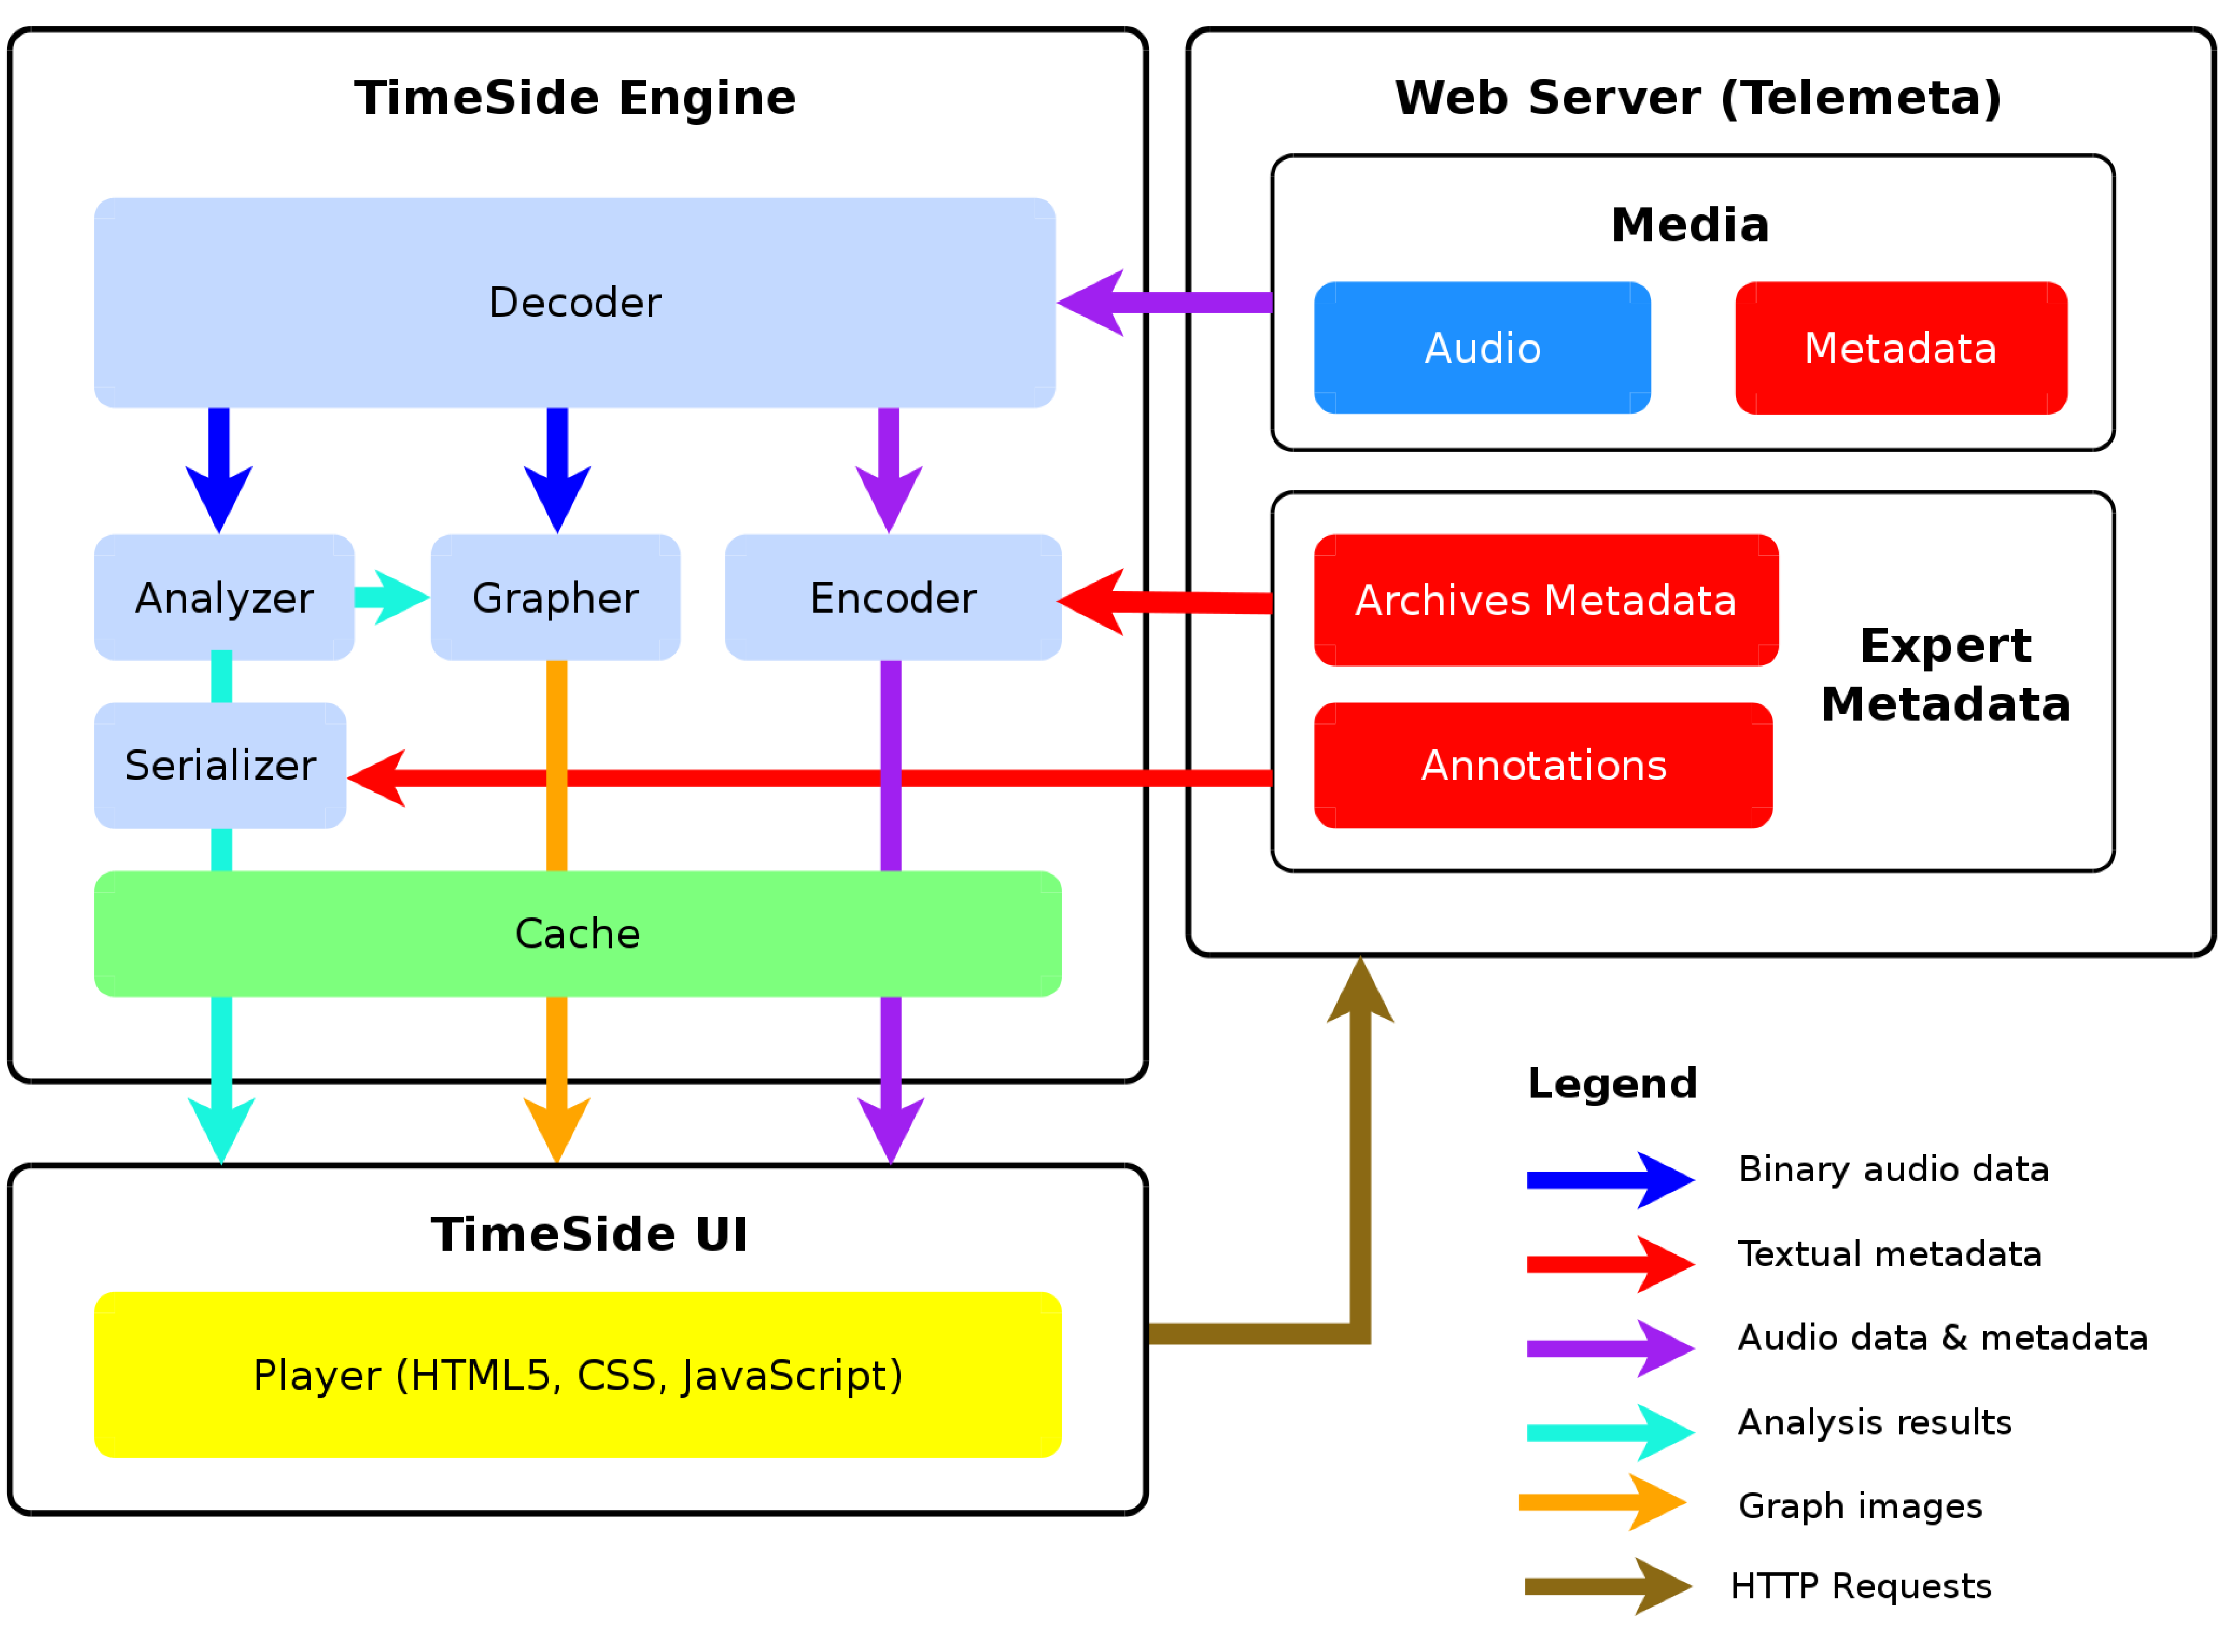
\includegraphics[width=0.8\textwidth]{img/timeside_schema_v3.pdf}
  \end{center}
\end{frame}

\subsection{Engine}

\begin{frame}
  \frametitle{TimeSide - Engine}
  \begin{center}
    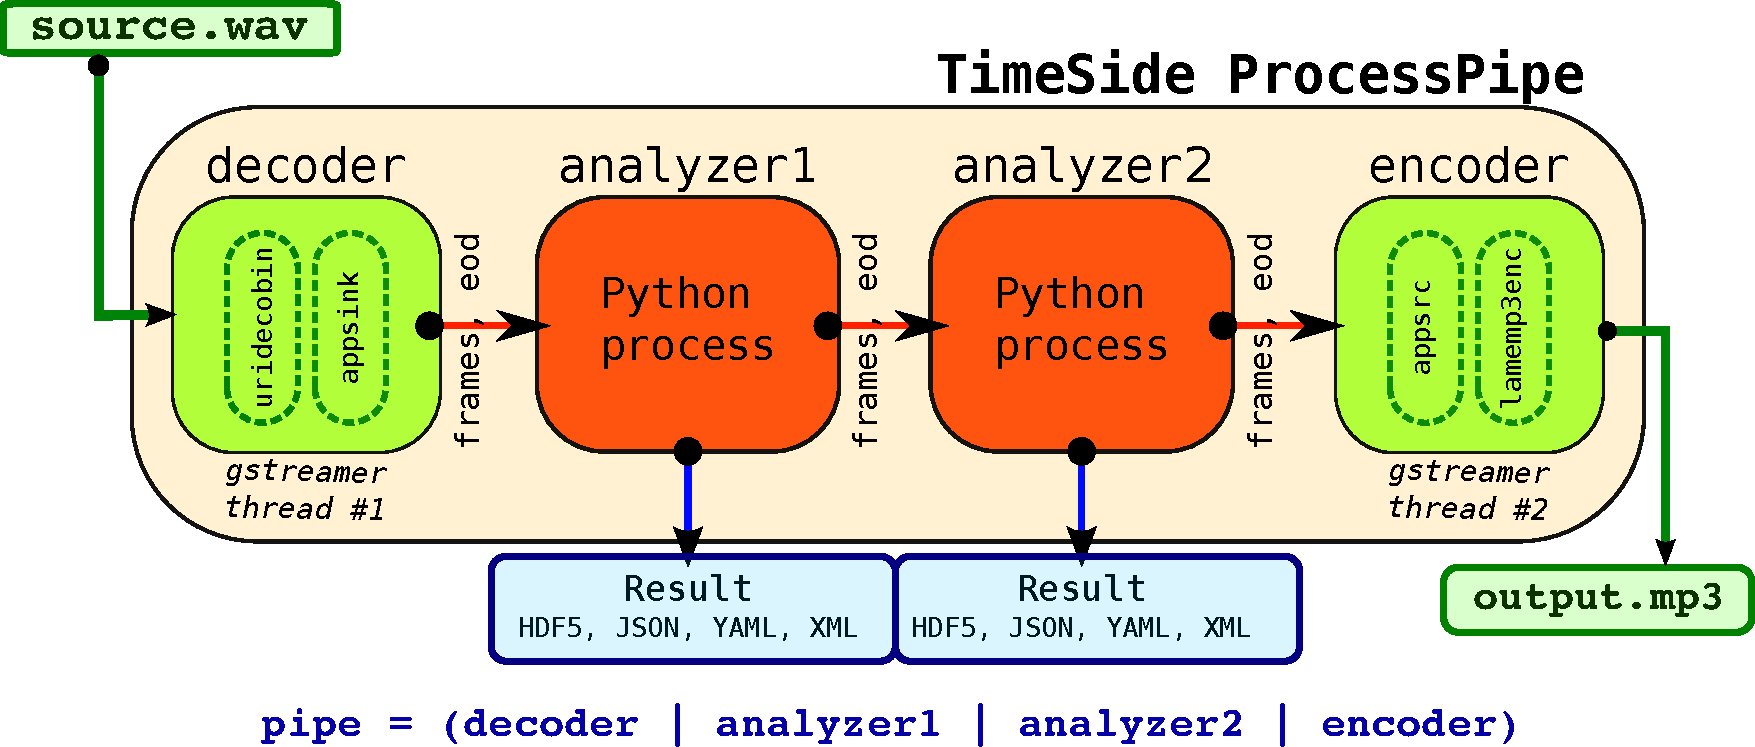
\includegraphics[width=0.95\textwidth]{img/TimeSide_pipe.pdf}
  \end{center}
  \begin{block}{Process Pipe}
    \begin{itemize}
    \item On-the-fly audio processing by simultaneous processors (decoder, encoders, analyzers, graphers)
    \item Use of \emph{Gstreamer} for audio decoding and encoding    \end{itemize}
  \end{block}
\end{frame}


\subsection{Processors}

\frame{\frametitle{Processors (plugins)}
    \begin{block}{Decoders}
        \begin{itemize}
        \item FileDecoder 
        \item ArrayDecoder
        \item LiveDecoder
       \end{itemize}
    \end{block}
    
    \begin{block}<2>{Encoders}
         \begin{itemize}
            \item VorbisEncoder
            \item WavEncoder
            \item Mp3Encoder
            \item FlacEncoder
            \item AacEncoder
            \item WebMEncoder
            \item OpusEncoder
            \item AudioSink
         \end{itemize}
    \end{block}
}

\frame{\frametitle{Processors (plugins)}
    \begin{block}{Analyzers}
        \begin{itemize}
        \item  AubioTemporal
        \item  AubioPitch
        \item  AubioMfcc
        \item  AubioMelEnergy
        \item  AubioSpecdesc
        \item  Yaafe
        \item  Spectrogram
        \item  Waveform
        \item  VampSimpleHost
        \item  IRITSpeechEntropy
        \item  IRITSpeech4Hz
        \item  OnsetDetectionFunction
        \item  LimsiSad
       \end{itemize}
    \end{block}
}

\frame{\frametitle{Processors (plugins)}
    \begin{block}{Graphers}
         \begin{itemize}
            \item Waveform
            \item WaveformCentroid
            \item WaveformTransparent
            \item WaveformContourBlack
            \item WaveformContourWhite
            \item SpectrogramLog
            \item SpectrogramLinear
            \item Display.aubio\_pitch.pitch
            \item Display.odf
            \item Display.waveform\_analyzer
            \item Display.irit\_speech\_4hz.segments
         \end{itemize}
    \end{block}
}

\subsection{Analyzer Result}
\begin{frame}
  \frametitle{Analyzer Result}
     \begin{block}{Result types: \\\emph{time mode} x \emph{data mode}}
       \begin{columns}
         \begin{column}{0.35\linewidth}
           \begin{itemize}
           \item Data modes:
             \begin{itemize}
             \item \alert<2-5>{Label}
             \item \alert<6-9>{Value}
             \end{itemize}
           \item Time modes:
             \begin{itemize}
             \item \alert<2,6>{Global}
             \item \alert<3,7>{Event}
             \item \alert<4,8>{Segment}
             \item \alert<5,9>{Framewise}
             \end{itemize}
           \end{itemize}
         \end{column}
         \begin{column}{0.50\linewidth}\footnotesize
           \begin{exampleblock}<2->{\footnotesize Result Container}\scriptsize
             \begin{itemize}
             \item ID Metadata
             \item Audio Metadata
             \item Parameters
             \item Data object
               \begin{itemize}\scriptsize
               \item<2-5> Label
               \item<2-5> Label Metadata ({\tiny label, label\_id, ...})
               \item<6-9> Value
               \item<3-4,7-8> Time
               \item<4,8> Duration
               \item<5,9> Frame Metadata ({\tiny sample rate, blocksize,
                 stepsize})
               \end{itemize}
           
             \end{itemize}
           \end{exampleblock}

         \end{column}
       \end{columns}
      
  \end{block}   
 \begin{block}<10>{Export}
         \begin{itemize}
         \item Serialization: HDF5, JSON, YAML, XML
         \item Display: \emph{Ad hoc} rendering methods (depending on time and data modes)
         \end{itemize}
       \end{block}
\end{frame}
\begin{frame}
\frametitle{Analyzer result examples}
\begin{center}
  \includegraphics<1>[width=\linewidth]{img/results/IRIT_Speech4Hz.png}
  \includegraphics<2>[width=\linewidth]{img/results/SOLO_DUOdetection.png}\\
  {\footnotesize \only<1>{\url{http://diadems.telemeta.org/archives/items/CNRSMH_I_2013_201_001_01/}}
  \only<2>{\url{http://diadems.telemeta.org/archives/items/CNRSMH_I_2000_008_001_04/}}}
\end{center}
\end{frame}
\section{Demos}

\frame{\frametitle{Documentation and demos}
    \begin{block}{Links}
         \begin{itemize}\small
            \item \chref{http://files.parisson.com/timeside/doc/}{Official documentation}
            \item \chref{http://nbviewer.ipython.org/github/thomasfillon/Timeside-demos/tree/master/}{Notebooks}
            \item \chref{http://archives.crem-cnrs.fr/archives/items/CNRSMH_I_1960_003_001_07/}{Online example 1}
            \item \chref{http://archives.crem-cnrs.fr/archives/items/CNRSMH_I_1976_011_003_08/}{Online Example 2}
            \item \chref{http://diadems.telemeta.org/archives/collections/?page=275&}{DIADEMS datasets}
         \end{itemize}
    \end{block}
}


\section{ToDo lists}

\frame{\frametitle{ToDo lists}
\footnotesize
\begin{block}{Telemeta}
    \begin{itemize}
    %\item Update code to support Django new Class based views
    \item Update web framework (DJANGO) and geolocation services
        %\item Smart breadcrumbs 
    %\item Better interactions with TimeSide
    \item Enhance user interface (full HTML 5 + web audio API)
        \begin{itemize}\footnotesize
            \item For annotations and segmentations in a collaborative manner
            \item Provide import capabilities and feedback loop between manual and automatic annotations
            \item Fancy displays of automatic analysis results (zoomable + synchronized with audio)
            \item Add a User interface to control and tune the analysis parameters
            \item Add public and enhanced user playlists
        \end{itemize}
    \item More documentation
    \end{itemize}
\end{block}

\begin{block}<2>{TimeSide}
    \begin{itemize}
    \item Tiny web server based on Django (done)
    \item Process task manager (done)
    %\item Full HTML5 zooming player (+ annotations, segmentations, etc..)
    %\item Analyzer parameters (+ interface)
    %\item Improve Vamp plugins support (Vamp python host ?)
    \item Add more audio \& acoustic analysis tools for automatic analysis
    \item Add more automatic segmentation and classification tools to support various semantic ontologies (cf. thesaurus)

    %\item Add automatic similarity analysis tools (inside a song or between sound items)
    %\item Enhance analysis result displays to send to Telemeta
    %\item \dchref{https://github.com/yomguy/TimeSide/issues}
    \end{itemize}
\end{block}
}

\section{Lessons}

\frame{\frametitle{Lessons learned}
\begin{block}{Lessons learned from a 7 years old project}
\begin{itemize}
\item Simplicity is better than complexity (\alert{KISS})
\item \alert{Modularity} is only accessible with a flexible language (thanks Python!)
\item \alert{Models} and \alert{Objects} are more important than Technologies
\item A good \alert{workflow} is defined by the users themselves through \alert{feedback} and constant revisions
\item \alert{Prototyping} is a crucial part of the development process
\item A good platform relies on \alert{standards}, not on formats
\item The \alert{Open Source} ecosystem gives some \alert{tremendous} possibilities to develop, deploy and scale any platform project
\end{itemize}
\end{block}
}


\frame{\frametitle{The End}
 \begin{center}
   \large{Thank you!}\\
   \large{We are looking for new collaborations\\ for large scale audio processing use cases. Let's keep in touch!}
   \vspace{0.25cm}
    \begin{block}{Links}
     \begin{itemize}\small
        \item \chref{http://github.com/yomguy/TimeSide}{github.com/yomguy/TimeSide}
        \item \chref{http://telemeta.org}{telemeta.org}
        \item \chref{https://twitter.com/telemeta/}{@telemeta}
    \end{itemize}
    \end{block}
    \begin{block}{Contact me}
    \begin{itemize}\small
    \item \chref{mailto:guillaume@parisson.com}{guillaume@parisson.com}
    \item \chref{https://twitter.com/yomguy/}{@yomguy}
    \item \chref{https://github.com/yomguy/}{github.com/yomguy/}
    \item \chref{https://plus.google.com/u/0/+GuillaumePellerin/posts}{+GuillaumePellerin}
    \item \chref{http://fr.linkedin.com/in/guillaumepellerin}{fr.linkedin.com/in/guillaumepellerin}
    \end{itemize}
     \end{block}
  \end{center}
}

\begin{frame}
  \frametitle{Web Audio Conference Announcement}

  \begin{center}
    WAC\\
 1st Web Audio Conference\\

    January 26-27, 2015 - IRCAM \& Mozilla Paris, France\\
    \textbf{\url{http://wac.ircam.fr/}}
  \end{center}

\emph{WAC is the first international conference on web audio technologies and applications.}

The conference welcomes web R\&D developers, audio processing scientists, application designers and people involved in web standards.

The conference addresses research, development, design, and standards concerned with emerging audio-related web technologies such as Web Audio API, Web RTC, Web Sockets, and Javascript. 

\begin{center}
  \emph{Deadline for submission: October 10, 2014}
\end{center}

\end{frame}
\end{document}